\documentclass[sigconf]{acmart}
\usepackage{algorithm}
\usepackage{caption}
\usepackage{algorithmicx}
\usepackage[noend]{algpseudocode}

%%
%% \BibTeX command to typeset BibTeX logo in the docs
\AtBeginDocument{%
  \providecommand\BibTeX{{%
    \normalfont B\kern-0.5em{\scshape i\kern-0.25em b}\kern-0.8em\TeX}}}

%% Rights management information.  This information is sent to you
%% when you complete the rights form.  These commands have SAMPLE
%% values in them; it is your responsibility as an author to replace
%% the commands and values with those provided to you when you
%% complete the rights form.
\setcopyright{acmcopyright}
\copyrightyear{2018}
\acmYear{2018}
\acmDOI{10.1145/1122445.1122456}

%% These commands are for a PROCEEDINGS abstract or paper.
\acmConference[Woodstock '18]{Woodstock '18: ACM Symposium on Neural
  Gaze Detection}{June 03--05, 2018}{Woodstock, NY}
\acmBooktitle{Woodstock '18: ACM Symposium on Neural Gaze Detection,
  June 03--05, 2018, Woodstock, NY}
\acmPrice{15.00}
\acmISBN{978-1-4503-XXXX-X/18/06}


%%
%% Submission ID.
%% Use this when submitting an article to a sponsored event. You'll
%% receive a unique submission ID from the organizers
%% of the event, and this ID should be used as the parameter to this command.
%%\acmSubmissionID{123-A56-BU3}

%%
%% The majority of ACM publications use numbered citations and
%% references.  The command \citestyle{authoryear} switches to the
%% "author year" style.
%%
%% If you are preparing content for an event
%% sponsored by ACM SIGGRAPH, you must use the "author year" style of
%% citations and references.
%% Uncommenting
%% the next command will enable that style.
%%\citestyle{acmauthoryear}

%%
%% end of the preamble, start of the body of the document source.
\begin{document}

%%
%% The "title" command has an optional parameter,
%% allowing the author to define a "short title" to be used in page headers.
\title{Context-Free Path Queries, Planar Graphs and Friends}

%%
%% The "author" command and its associated commands are used to define
%% the authors and their affiliations.
%% Of note is the shared affiliation of the first two authors, and the
%% "authornote" and "authornotemark" commands
%% used to denote shared contribution to the research.

\author{Alexandra Istomina}
\affiliation{%
  \institution{The Th{\o}rv{\"a}ld Group}
  \streetaddress{1 Th{\o}rv{\"a}ld Circle}
  \city{Hekla}
  \country{Iceland}}
\email{larst@affiliation.org}

\author{Alexandra Olemskaya}
\affiliation{%
  \institution{Inria Paris-Rocquencourt}
  \city{Rocquencourt}
  \country{France}
}

\author{Ekaterina Shemetova}
\affiliation{%
  \institution{Inria Paris-Rocquencourt}
  \city{Rocquencourt}
  \country{France}
}


\author{Semyon Grigorev}
\affiliation{%
 \institution{Rajiv Gandhi University}
 \streetaddress{Rono-Hills}
 \city{Doimukh}
 \state{Arunachal Pradesh}
 \country{India}}



%%
%% By default, the full list of authors will be used in the page
%% headers. Often, this list is too long, and will overlap
%% other information printed in the page headers. This command allows
%% the author to define a more concise list
%% of authors' names for this purpose.

%%
%% The abstract is a short summary of the work to be presented in the
%% article.
\begin{abstract}

Abstract is very abstract.

\end{abstract}

%%
%% The code below is generated by the tool at http://dl.acm.org/ccs.cfm.
%% Please copy and paste the code instead of the example below.
%%
\begin{CCSXML}
<ccs2012>
 <concept>
  <concept_id>10010520.10010553.10010562</concept_id>
  <concept_desc>Computer systems organization~Embedded systems</concept_desc>
  <concept_significance>500</concept_significance>
 </concept>
 <concept>
  <concept_id>10010520.10010575.10010755</concept_id>
  <concept_desc>Computer systems organization~Redundancy</concept_desc>
  <concept_significance>300</concept_significance>
 </concept>
 <concept>
  <concept_id>10010520.10010553.10010554</concept_id>
  <concept_desc>Computer systems organization~Robotics</concept_desc>
  <concept_significance>100</concept_significance>
 </concept>
 <concept>
  <concept_id>10003033.10003083.10003095</concept_id>
  <concept_desc>Networks~Network reliability</concept_desc>
  <concept_significance>100</concept_significance>
 </concept>
</ccs2012>
\end{CCSXML}

\ccsdesc[500]{Computer systems organization~Embedded systems}
\ccsdesc[300]{Computer systems organization~Redundancy}
\ccsdesc{Computer systems organization~Robotics}
\ccsdesc[100]{Networks~Network reliability}

%%
%% Keywords. The author(s) should pick words that accurately describe
%% the work being presented. Separate the keywords with commas.
\keywords{datasets, neural networks, gaze detection, text tagging}


%%
%% This command processes the author and affiliation and title
%% information and builds the first part of the formatted document.
\maketitle
\chapter*{Введение}                         % Заголовок
\addcontentsline{toc}{chapter}{Введение}    % Добавляем его в оглавление
\textbf{Актуальность работы}

Статический анализ исходного кода является известной техникой  получения знаний о программе без её исполнения ~\cite{StaticCodeAnalysis3,StaticCodeAnalysis2,StaticCodeAnalysis1}. Статический анализ является неотъемлемой частью многих процессов, связанных с разработкой программного обеспечения (ПО), и может использоваться, например, для упрощения работы с кодом с помощью подсветки синтаксиса языка в программах, навигации по коду, реализации контекстных подсказок. Более того, статический анализ используется для обнаружения ошибок на ранних стадиях разработки, до запуска программы, а также для поиска различных семантических ошибок, которые не могут быть определены обычным синтаксическим анализом.  Также, статический анализ используется при решении задач трансформации исходного кода и реинжиниринге~\cite{reengANT}. Однако во многих языках программирования имеются конструкции, которые существенно затрудняют статический анализ. 

Например, широко используются динамические встроенные языки --- приложение, созданное на одном языке, генерирует программу на другом языке и передаёт её на выполнение в соответствующее окружение. Примерами могут служить динамические SQL-запросы к базам данных из приложений на Java, С++, С\#, формирование HTML-страниц в PHP-приложениях~\cite{DSQLISO,JSP,PHPmySQL}. Генерируемый код собирается из строк таким образом, чтобы в момент выполнения результирующая строка представляла собой корректную программу. Примеры использования встроенных языков представлены в листингах~\ref{lst:dsql1},~\ref{lst:JsJava} и~\ref{lst:PhPSqlHtml}. Следует отметить, что одна программа может генерировать код на нескольких языках (см. листинг~\ref{lst:PhPSqlHtml}). При этом возможно получение частей кода из разных источников (например, учитывать текстовый ввод пользователя, что часто используется для задания фильтров при конструировании SQL-запросов). Использование динамически формируемых программ  позволяет избежать дополнительных накладных расходов, присущих таким технологиям, как ORM\footnote{ORM или Object-Relational Mapping --- технология программирования, которая связывает базы данных с концепциями объектно-ориентированных языков программирования~\cite{ORM}.}, и достичь высокой производительности. Благодаря этому использование динамически генерируемых программ получило широкое распространение и применяется до сих пор. Вместе с этим, несмотря на появление новых технологий, динамическая генерация SQL-запросов активно используется и в настоящее время~\cite{DSQLInActiveUse}.

\fvset{frame=lines,framesep=5pt,fontsize=\small}\

\begin{listing}
    \begin{pyglist}[language=sql,numbers=left,numbersep=5pt]

CREATE PROCEDURE [dbo].[MyProc]  @TABLERes   VarChar(30)
AS
    EXECUTE ('INSERT INTO ' + @TABLERes + ' (sText1)' +
             ' SELECT ''Additional condition: '' + sName' +
             ' from #tt where sAction = ''1000000''')
GO
    \end{pyglist}
\caption{Код с использованием динамического SQL}
\label{lst:dsql1}
\end{listing} 
 
\fvset{frame=lines,framesep=5pt}
\begin{listing}
    \begin{pyglist}[language=java,numbers=left,numbersep=5pt]
import javax.script.*;  
public class InvokeScriptFunction {  
    public static void main(String[] args) throws Exception {  
        ScriptEngineManager manager = new ScriptEngineManager();  
        ScriptEngine engine = manager.getEngineByName("JavaScript");  
        // JavaScript code in a String  
        String script = 
            "function hello(name) { print('Hello, ' + name); }";  
        // evaluate script  
        engine.eval(script);  
        // javax.script.Invocable is an optional interface.  
        // Check whether your script engine implements or not!  
        // Note that the JavaScript engine implements
        // Invocable interface.  
        Invocable inv = (Invocable) engine;  
        // invoke the global function named "hello"  
        inv.invokeFunction("hello", "Scripting!!" );  
    }  
}
    \end{pyglist}
\caption{Вызов JavaScript из Java}
\label{lst:JsJava}
\end{listing}


\fvset{frame=lines,framesep=5pt}
\begin{listing}
    \begin{pyglist}[language=php,numbers=left,numbersep=5pt]

<?php
    // Embedded SQL
    $query = 'SELECT * FROM ' . $my_table; 
    $result = mysql_query($query);
    
    // HTML markup generation
    echo "<table>\n";
    while ($line = mysql_fetch_array($result, MYSQL_ASSOC)) {
        echo "\t<tr>\n";    
        foreach ($line as $col_value) {
            echo "\t\t<td>$col_value</td>\n";
        }
        echo "\t</tr>\n";
    }
    echo "</table>\n";
?>
    \end{pyglist}
\caption{Использование нескольких встроенных в PHP языков (MySQL, HTML)}
\label{lst:PhPSqlHtml}
\end{listing}



Динамически формируемые выражения часто конструируются с помощью таких операций, как конкатенация в циклах или условных предложениях, или в рекурсивных процедурах. Это затрудняет статический анализ и приводит к получению множества возможных значений для каждого выражения в момент выполнения. Вследствие этого фрагменты динамически формируемого кода воспринимаются компилятором исходного языка как простые строки, не подлежащие дополнительному анализу, а это, в свою очередь, приводит к высокой вероятности возникновения ошибок во время выполнения программы. В худшем случае такая ошибка не приведёт к прекращению работы приложения, что указало бы на проблемы, однако целостность данных при этом может оказаться нарушена. Более того, использование динамически формируемых выражений затрудняет не только разработку информационных систем, так и также и реинжиниринг, поскольку в последнем случае важно автоматизировать перенос системы на новые зыки и платформы, что невозможно без качественного статического анализа. Например, при наличии в коде приложения динамически формируемых SQL-запросов нельзя точно ответить на вопрос о том, с какими элементами базы данных не взаимодействует система, и удалить их. При переносе такой системы на другую СУБД необходимо гарантировать, что для всех динамически формируемых выражений значение в момент выполнения будет корректным кодом на языке новой СУБД~\cite{JSquash}. Следует отметить, что отсутствие статического анализа динамически формируемых программ не позволяет реализовывать для них стандартную функциональность интегрированных сред разработки (Integrated Development Environment, IDE) --- подсветку синтаксиса и автодополнение, рефакторинг кода и т.д. Такая функциональность значительно упрощает процесс разработки и отладки приложений и полезна не только для основного языка, но и для встроенных языков. 

Для решения всех перечисленных выше задач необходимы инструменты, проводящие статический анализ динамически формируемых программ. Такой анализ может дать существенную информацию о таких программах, поскольку редко встречается ситуация полной динамической неопределённости (например, при создании динамических программ исключительно на основе пользовательского ввода). В большинстве случаев, имея программу, генерирующую динамические вставки, с помощью статического анализа можно получить достаточно информации для решения поставленных выше задач. Решению этой проблемы и посвящена данная диссертационная работа. 


\textbf{Степень разработанности темы}

Существуют классические исследования, посвященные разработке компиляторов --- работы А.~Ахо~\cite{Dragon}, А.~Брукера~\cite{CompilerCompiler}, С.~Джонсона~\cite{yaccBook},  Б.К.Мартыненко~\cite{Martinenko1, Martinenko2}  и др.  Однако содержащиеся там алгоритмы синтаксического анализа не могут быть применены к решению задачи анализа динамически формируемых программ, поскольку предназначены для обработки входных данных, представимых в видн линейной последовательности символов, а такое представление динамически формируемых программ не всегда возможно.

Методы обобщённого синтаксического анализа, лежащие в основе данной работы, изложены в трудах таких учёных как Масару Томита (Masaru Tomita)~\cite{Tomita}, Элизабет Скотт (Elizabeth Scott) и Адриан Джонстон (Adrian Johnstone)~\cite{RNGLR,RIGLR} из университета Royal Holloway (Великобритания), Ян Рекерс (Jan Rekers, University of Amsterdam)~\cite{SPPF}, Элко Виссер (Eelco Visser)~\cite{RNGLRSyntaxerror2,RNGLRSyntaxerror3} и других.

Анализу динамически формируемых строковых выражений посвящены работы таких зарубежных учёных как Кюнг-Гу Дох (Kyung-Goo Doh)~\cite{LrAbstract1,LrAbstract2,LRAbstractParsingSema}, Ясухико Минамиде (Minamide Yasuhiko)~\cite{PHPSA}, Андерс Мёллер (Anders M{\o}ller)~\cite{JSA} и отечественных учёных А.А.~Бреслава~\cite{Alvor1,Alvor2} и других. Хорошо изучены вопросы проверки корректности динамически формируемых выражений и поиска фрагментов кода, уязвимых для SQL-инъекций~\cite{SQLInjection,Dasgupta:2009:SAF:1546683.1547548}. Однако данные работы исследуют отдельные аспекты проблемы статического анализа динамически формируемых программ, оставляя в стороне создание готовых алгоритмов (в частности, не строят структурное представление анализируемых программ). В связи с этим возникают проблемы масштабируемости данных результатов, например, создание на их основе более сложных видов статического анализа.

Так же важным является предоставление компонентов, упрощающих создание новых инструментов для решения конкретных задач. Данных подход хорошо исследован в области разработки компиляторов, где широкое распространение получили генераторы анализаторов и пакеты стандартных библиотек (работы А.~Ахо~\cite{Dragon}, А.~Брукера~\cite{CompilerCompiler}, С.~Джонсона~\cite{yaccBook} и др.). 

В работах отечественных учёных М.Д.~Шапот и Э.В.~Попова~\cite{DynamicDSQLTranslation}, а так же зарубежных учёных Антони Клеви (Anthony Cleve), Жан-Люк Эно (Jean-Luc Hainaut)~\cite{DSQLReverseEngineering}, Йост Виссер (Joost Visser)~\cite{DSQLQualityMesure} и других рассматриваются различные аспекты реинжиниринга информационных систем, использующих встроенные SQL-запросы, однако не формулируется общего метода для решения таких задач. Этот вопрос также не затрагивается в классических работах, посвященных реинжиниригу~\cite{SoftwareReeng1, reengANT, SoftwareReeng2, SoftwareReeng3}. Однако разработка такого метода является актуальной задачей.

Таким образом, актуальной является задача дальнейшего исследования статического анализа динамически формируемых строковых выражений. Кроме этого важным является решение вопросов практического применения средств анализа динамически формируемого кода: упрощение разработки инструментов анализа и создание методов их применения в реинжиниринге программного обеспечения.
\textbf{Объект исследования}

Объектом исследования являются методы, алгоритмы и программные средства обработки динамически формируемых программ, а также задача реинжиниринга информационных систем.

\textbf{Цель и задачи диссертационной работы}

\textbf{Целью} данной работы является создание комплексного подхода к статическому синтаксическому анализу динамически формируемых программ.

Достижение поставленной цели обеспечивается решением следующих \textbf{задач}.
\begin{enumerate}
    \item Разработать универсальный алгоритм синтаксического анализа динамически формируемых программ, не зависящий от целевого языка программирования и допускающий реализацию различных видов статического анализа. 
    \item Создать архитектуру инструментария для автоматизации разработки программных средств статического анализа динамически формируемых программ.
    \item Создать метод реинжиниринга динамически формируемых программ.
\end{enumerate}

\textbf{Методология и методы исследования}

Методология исследования основана на подходе к спецификации и анализу формальных языков, активно развивающемуся с 50-х годов 20-го века (см., например, работы Н. Хомского~\cite{chomskyMethod ,chomskySyntactic}). В последствии этот подход получил широкое распространение в областях, связанных с обработкой языков программирования.
Основными элементами данного подхода являются алфавит и грамматика языка, разбиение автоматической обработки языка на выполнение таких шагов как лексический, синтаксический и семантический анализ. Решаемые в связи с этим задачи связаны с поиском эффективных алгоритмов, выполняющих эти шаги. 

В работе применяется алгоритм обобщённого восходящего синтаксического анализа RNGLR~\cite{RNGLR}, созданный Элизабет Скотт (Elizabeth Scott) и Адриан Джонстон (Adrian Johnstone) из университета Royal Holloway (Великобритания). Для компактного хранения леса вывода использовалась структура данных Shared Packed Parse Forest (SPPF), которую предложил Ян Рекерс (Jan Rekers, University of Amsterdam)~\cite{SPPF}.

Доказательство завершаемости и корректности предложенного алгоритма проводилось с применением теории формальных языков, теории графов и теории сложности алгоритмов. Приближение множества значений динамически формируемого выражения строилось в виде регулярного множества, описываемого с помощью конечного автомата.


\textbf{Положения, выносимые на защиту}
\begin{enumerate}
    \item Разработан алгоритм синтаксического анализа динамически формируемых программ, позволяющий обрабатывать произвольную регулярную аппроксимацию множества значений выражения в точке выполнения, реализующий эффективное управление стеком и гарантирующий конечность представления леса вывода. Доказана завершаемость и корректность предложенного алгоритма при обработке регулярной аппроксимации, представимой в виде произвольного конечного автомата без $\varepsilon$-переходов. 
    \item Создана архитектура инструментария для разработки программных средств статического анализа динамически формируемых программ.
    \item Разработан метод анализа и обработки динамически формируемых программ в проектах по реинжинирингу информационных систем. 
\end{enumerate}

\textbf{Научная новизна работы}

Научная новизна полученных в ходе исследования результатов заключается в следующем.

\begin{enumerate}

\item Алгоритм, предложенный в диссертации, отличается от аналогов (работы Андрея Бреслава~\cite{Alvor1, Alvor2}, Кюнг-Гу Дох~\cite{LrAbstract1, LrAbstract2}, Ясухико Минамиде~\cite{PHPSA}) возможностью построения компактной структуры данных, содержащей деревья вывода для всех корректных значений выражения. Это позволяет использовать результаты работы алгоритма для проведения более сложных видов анализа. Алгоритмы, представленные в (JSA~\cite{JSA}~\cite{Alvor1, Alvor2}, PHPSA~\cite{PHPSA}) предназначены только для проверки корректности выражений, основанной на решении задачи о включении одного языка в другой. Выполнение более сложных видов анализа, трансформаций или построения леса разбора не предполагается. 

\item Новизна представленной архитектуры заключается в том, что она позволяет создать платформу для разработки целевых инструментов, решающих широкий круг задач анализа динамически формируемого кода. Существующие архитектуры готовых инструментов (JSA, PHPSA, Alvor, Varis) предназначены для решения конкретных задач для определённых языков. Решение новых задач или поддержка других языков с помощью этих инструментов затруднены ввиду ограничений, накладываемых архитектурой и возможностями используемого алгоритма анализа. 

\item Метод анализа и обработки встроенного программного кода в проектах по реинжинирингу информационных систем предложен впервые. К.В.~Ахтырченко и Т.П.~Сорокваша отмечают~\cite{SoftwareReengMethods}, что существующие работы в области реинжиниринга программного обеспечения либо содержат высокоуровневые решения, не касающиеся деталей, важных при решении прикладных задач (например, работы К. Вагнера~\cite{SoftwareReeng3}, Х. Миллера~\cite{SoftwareReeng2}), либо являются набором подходов к решению конкретных задач (например, работы~\cite{SoftwareReeng1, reengANT, boulychev}). При этом, встроенный программный код часто не учитывается. С другой стороны, работы М.Д.~Шапот и Э.В.~Попова~\cite{DynamicDSQLTranslation}, С.Л.~Трошина~\cite{reengANT}, А.~Клеви~\cite{DSQLReverseEngineering}  посвящены решению конкретных задач обработки встроенного программного кода в контексте реинжиниринга информационных систем, но не предлагают обобщённого и масштабируемого метода.

\end{enumerate}


\textbf{Теоретическая и практическая значимость работы}

Теоретическая значимость диссертационного исследования заключается в разработке формального алгоритма синтаксического анализа динамически формируемого кода, решающего задачу построения конечного представления леса вывода, не решенную полностью ранее, а также в формальном доказательстве завершаемости и корректности разработанного алгоритма. 

На основе полученных в работе научных результатов был разработан инструментарий (Software Development Kit, SDK), предназначенный для создания средств статического анализа динамически формируемых программ. 
С использованием разработанного инструментария было реализовано расширение к инструменту ReSharper (ООО ``ИнтеллиДжей Лабс'', Россия), предоставляющее поддержку встроенного T-SQL в проектах на языке программирования C\# в среде разработки Microsoft Visual Studio. Так же было выполнено внедрение результатов работы в промышленный проект по переносу хранимого SQL-кода с MS-SQL Server 2005 на Oraclе 11gR2 (ЗАО ``Ланит-Терком'', Россия). 

\textbf{Степень достоверности и апробация результатов}

Достоверность и обоснованность результатов исследования опирается на использование формальных методов исследуемой области, проведенные доказательства, рассуждения и эксперименты.

Основные результаты работы были доложены на ряде научных конференций: SECR-2012, SECR-2013, SECR-2014, TMPA-2014, Parsing@SLE-2013, Рабочий семинар ``Наукоемкое программное обеспечение'' при конференции PSI-2014. Доклад на SECR-2014 награждён премией Бертрана Мейера за лучшую исследовательскую работу в области программной инженерии. Дополнительной апробацией является то, что разработка инструментальных средств на основе предложенного алгоритма была поддержана Фондом содействия развитию малых форм предприятий в технической сфере (программа УМНИК~\cite{UMNIC}, проекты \textnumero~162ГУ1/2013 и \textnumero~5609ГУ1/2014).

\textbf{Публикации по теме диссертации}

Все результаты диссертации изложены в 7 научных работах, из которых 3~\cite{YCArticle,SELforIDEru,AbstractGLL}, содержащие основные результаты, опубликованы в журналах из ‘’Перечня российских рецензируемых научных журналов, в которых должны быть опубликованы основные научные результаты диссертаций на соискание ученых степеней доктора и кандидата наук’’, рекомендовано ВАК. 
1 работа~\cite{GLRAbsPars} индексируются Scopus. В работах, написанных в соавторстве, вклад автора определяется следующим образом.  В~\cite{Syrcose} С. Григорьеву принадлежит реализация ядра платформы YaccConstructor. В~\cite{SELforIDEru, AbstractGLL} и~\cite{SELforIDE} С. Григорьеву принадлежит постановка задачи, формулирование требований к разрабатываемым инструментальным средствам, работа над текстом. 
В~\cite{GLRAbsPars} автору принадлежит идея, описание и реализация анализа встроенных языков на основе RNGLR алгоритма.  В~\cite{YCArticle} С. Григорьеву принадлежит реализация инструментальных средств, проведение экспериментов, работа над текстом. В работе~\cite{RelaxedARNGLR} автору принадлежит алгоритм синтаксического анализа динамически формируемого кода.


\textbf{Структура работы}

Диссертация состоит из введения, шести глав, заключения и построена следующим образом. В первой главе приводится обзор области исследования. Рассматриваются подходы к анализу динамически формируемых строковых выражений и соответствующие инструменты. Описывается алгоритм обобщённого восходящего синтаксического анализа RNGLR, взятый за основу в диссертационной работе. Также описываются проекты YaccConstructor и ReSharper SDK, использованные для реализации предложенного в работе инструментария. Во второй главе формализуется основная задача исследования и излагается решающий её алгоритм синтаксического анализа регулярных множеств. Приводится доказательство завершаемости и корректности представленного алгоритма, приводятся примеры. В третьей главе описывается инструментальный пакет YC.SEL.SDK, разработанного на основе алгоритма, описанного во второй главе и предназначеного для разработки инструментов анализа динамически формируемых программ. Описывается архитектура компонентов и особенности их реализации. Также описывается YC.SEL.SDK.ReSharper --- ``обёртка'' для YC.SEL.SDK, позволяющая создавать расширения к ReSharper для поддержки встроенных языков. В четвёртой главе описывается метод реинжиниринга встроенного программного кода.  В пятой главе приводятся результаты экспериментального исследования разработанного алгоритма и инструмента YC.SEL.SDK. Шестая глава содержит результаты сравнения и соотнесения полученных результатов с  существующими аналогами.

\textbf{Благодарности}

А.Н.Терехову, работкникам и администрации компании ЗАО ``Ланит-Терком'' за создания условий для изучения данной темы (организация проектов по реинжинирингу). Я.А.Кириленко за погружение в тему исследования и руководство на начальных этапах. Д.Ю.Булычеву за помощь в уточнении постановки задачи исследования и в написании статей. Студентам и аспирантам кафедры системного программирования Дмитрию Авдюхину, Анастасии Рагозиной, Екатерине Вербицкой, Марине Полубеловой, Иванову Андрею за помощь в реализации предложенных идей и проведение экспериментов. Отдельную благодарность  хочется выразить компании ООО ``ИнтеллиДжей Лабс'' и Андрею Иванову за поддержку исследований. Также хочется поблагодарить А.К.Петренко и В.М.Ицыксона, а также сотрудников ИСП РАН за ценные вопросы и комментарии к работе, позволившие уточнить ряд формулировок и улучшить изложение результатов. 

\section{Preliminaries} \label{section_preliminaries}
In this section, we introduce the basic notions used throughout the paper.

Let $\Sigma$ be a finite set of edge labels. Define an \textit{edge-labeled directed graph} as a tuple $D = (V, E)$ with $V$ is a set of nodes and $E \subseteq V \times \Sigma \times V$ is a directed edge-relation.  For a path $\pi$ in a graph $D$ we denote $l(\pi)$ --- the unique word obtained by concatenating the labels of the edges along the path $\pi$. Also, we write $n \pi m$ to indicate that a path $\pi$ starts at node $n \in V$ and ends at node $m \in V$.

According to Hellings~\cite{hellingsRelational}, we deviate from the usual definition of a context-free grammar in \textit{Chomsky Normal Form}~\cite{chomsky} by not including a special start non-terminal, which will be specified in the queries to the graph. Since every context-free grammar can be transformed into an equivalent one in Chomsky Normal Form and checking that an empty string is in the language is trivial, then it is sufficient to only consider grammars of the following type. A \textit{context-free grammar} is 3-tuple $G = (N, \Sigma, P)$ where $N$ is a finite set of non-terminals, $\Sigma$ is a finite set of terminals, and $P$ is a finite set of productions of the following forms:

\begin{itemize}
    \item $A \rightarrow B C$, for $A,B,C \in N$,
    \item $A \rightarrow x$, for $A \in N$ and $x \in \Sigma$.   
\end{itemize}

Note that we omit the rules of the form $A \rightarrow \varepsilon$, where $\varepsilon$ denotes an empty string. This does not limit the applicability of further algorithms because checking that an empty string belongs to the context-free language in Chomsky normal form is trivial and only the empty paths $m \pi m$ correspond to an empty string $\varepsilon$.

We use the conventional notation $A \xrightarrow{*} w$ to denote that the string $w \in \Sigma^*$ can be derived from a non-terminal $A$ by some sequence of applying the production rules from $P$. The \textit{language} of a grammar $G = (N,\Sigma,P)$ with respect to a start non-terminal $S \in N$ is defined by $L(G_S) = \{w \in \Sigma^*~|~S \xrightarrow{*} w\}$.

For a given graph $D = (V, E)$ and a context-free grammar $G = (N, \Sigma, P)$, we define \textit{context-free relations} $R_A \subseteq V \times V$, for every $A \in N$, such that $R_A = \{(n,m)~|~\exists n \pi m~(l(\pi) \in L(G_A))\}$.

We define a binary operation on arbitrary subsets $N_1 , N_2$ of $N$ with respect to a context-free grammar $G = (N, \Sigma, P)$ as $N_1 \cdot N_2 = \{A~|~\exists B \in N_1, \exists C \in N_2 \text{ such that }(A \rightarrow B C) \in P\}.$

Using this binary operation as a multiplication on arbitrary subsets of $N$ and union of sets as an addition, we can define a \textit{matrix multiplication}, $a \cdot b = c$, where $a$ and $b$ are matrices of the suitable size that have subsets of $N$ as elements, as $c_{i,j} = \bigcup^{n}_{k=1}{a_{i,k} \cdot b_{k,j}}$.

We define the \textit{transitive closure} of a square matrix $a$ as $a^+ = a^{(1)} \cup a^{(2)} \cup \cdots$ where $a^{(i)} = a^{(i-1)} \cup (a^{(i-1)} \cdot a^{(i-1)})$, $i \ge 2$ and $a^{(1)} = a$.
\section{CFPQ on planar digraphs}

\subsection{Dynamic transitive closure}

We want to consider algorithms for semi-dynamic transitive closure for the case of a planar graph. Our algorithm needs to support only edge insertions that do not violate planarity.

There are several algorithms that look into the problem of dynamic reachability in planar digraphs and have sublinear both update and query time~\cite{10.5555/647903.739284},~\cite{karczmarz2018data},~\cite{kao2008encyclopedia}. 

Some algorithms~\cite{10.5555/1778580.1778635},~\cite{karczmarz2018data} restrict insertions to only that edges that respect the specific embedding of the planar graph. 

\todo[inline]{maybe we can choose one embedding at random and hope that nothing will violate it. So it will be monte-carlo (why it will have good probability? where from can we get all the possible non-isomorphic embeddings?)}  

The algorithms that allow edge insertions not with respect to the embedding of the graph, but to the planarity, are described in~\cite{10.5555/647903.739284},~\cite{10.1145/300515.300517}. The main idea of both articles is the same: a planar graph is separated into \textit{clusters} (edge induced subgraphs) for which reachability is shown by their sparse substitute $S$. \textit{Sparse substitute} is a graph that contains the reachability information between some set of vertices that lie in the same face of an embedded graph.

We show the results of~\cite{10.5555/647903.739284} more closely as they differ from the results of~\cite{10.1145/300515.300517} only by a logarithmic factor, have the same idea and are easier for understanding. 

Updates and queries are the following: adding or deleting the edge between vertices $u, v$, checking reachability, checking if new edge $(u, v)$ violates planarity. 

Every update procedure modifies a constant number of clusters, for which we reconstruct their sparse substitutes. If the procedure added the edge, new edge forms its own cluster. Moreover after every $\mathcal{O}(n^{1/3})$ insertions we rebuild cluster partition and sparse substitutes from the scratch so that clusters do not lose their properties, this rebuilding time is distributed between these $\mathcal{O}(n^{1/3})$ insertions, so insertion time is amortized. 

After splitting graph into clusters and looking into its sparse substitute update or query about vertices $u, v$ can be done by placing clusters of the vertices $u, v$ in the original graph $G$ into the graph of sparse substitutes $S$.

For maintaining dynamic transitive closure in this way we only need planarity to divide graph $G$ into clusters and for each cluster to build its sparse substitute. As we rebuild cluster partition and substitutes at the beginning and after every $\mathcal{O}(n^{\frac{1}{3}})$ edge-insertions, graph needs to remain planar during the updates. 

The results are the following.
 
\begin{enumerate}
	\item The amount of time for preprocessing is $\mathcal{O}(n \log n)$ --- in this time we find the separation of the given graph $G$ into $\mathcal{O}(n^{\frac{1}{3}})$ clusters (each consists of no more than $n^{\frac{2}{3}}$ edges of $G$) and build sparse substitution graph $S$ of total size $\mathcal{O}(n^{\frac{2}{3}} \log n)$ for them.
	
	\item After that we can perform add operation in $\mathcal{O}(n^{\frac{2}{3}} \log n)$ amortized time, delete operation in $\mathcal{O}(n^{\frac{2}{3}} \log n)$ worst-case time.
	
	\item Reachability query takes $\mathcal{O}(n^{\frac{2}{3}} \log n)$ worst-case time.
	
	\item Checking if the graph is planar can be done in $\mathcal{O}(n^{\frac{1}{2}})$ amortized time. 
\end{enumerate}

Let us look closely on how can we use the power of sparse substitution on our incremental transitive closure problem.

\begin{proposition}
We can maintain the structure described in~\cite{10.5555/647903.739284} not only for planar graphs, but for planar graphs with $\mathcal{O}(n^{\frac{1}{3}})$ edges that violate planarity. 
\end{proposition}

$\square$
In~\cite{10.5555/647903.739284} the number of clusters is $\mathcal{O}(n^{\frac{1}{3}})$. In the beginning and after every $\mathcal{O}(n^{\frac{1}{3}})$ edge insertions we rebuild sparse substitute graph $S$. and in these moments we need planarity. We can additionally maintain the set of non-planar edges, each edge of this set will present its own cluster and will not take part in the rebuilding of sparse substitution. Edge is \textit{non-planar} if its insertion to current planar graph $G$ makes it non-planar.
$\hfill\blacksquare$

\begin{proposition}
We can add edges in the graph and print out new pairs of reachable vertices for every insertion in $\mathcal{O}(n^{\frac{5}{3}})$ total time for every sequence of insertions if our model allows parallel computations.
\end{proposition}

$\square$
From~\cite{10.5555/647903.739284} we can add an edge $(u, v)$ in $\mathcal{O}(n^{\frac{2}{3}}\log n)$ amortized time. We want to get all pairs of vertices that are connected through the new edge.

We can run DFS from $v$ and DFS on reversed edges from $u$ in graph $S$ of sparse substitutes. DFS runs in time proportional to the size of the graph $S$ --- $\mathcal{O}(n^{\frac{2}{3}} \log n)$. After that for every cluster in the original graph $G$ we create dummy vertex $s$ and edges from $s$ to all boundary vertices in the cluster that were reached from $u$ and $v$ respectively. Then run DFS from this dummy vertex $s$. We print out every vertex that was reached by our DFSs, so we get two lists $U$ and $V$ for beginnings and the endings of the paths, going through $(u, v)$.

If any vertex $w$ is reachable from $v$ (without loss of generation), then it is a boundary vertex or lie in some cluster and is reachable from some boundary vertex of this cluster. In both cases, one of DFS's will print it out and the algorithm is correct. 

If we can run these DFS's in parallel (there are $\mathcal{O}(n^{\frac{1}{3}})$ clusters and the same number of DFS's), then each of them will take $\mathcal{O}(n^{\frac{2}{3}})$ amount of time (all cluster have $\mathcal{O}(n^{\frac{2}{3}})$ edges by definition in~\cite{10.5555/647903.739284}). As maximum number of edges in the planar graph is linear, the total amount of time will be $\mathcal{O}(n^{\frac{5}{3}})$ for every sequence of edge insertions.
$\hfill\blacksquare$

\begin{conjecture}
If our model does not allow parallel computations total amount of time for every sequence of insertions is at most $\mathcal{O}(n^2)$ and planarity does not get us any advantage in solving the problem of dynamic reachability (in amortized time per edge and query).
\end{conjecture}

[Thoughts]
If our model can not run algorithms in parallel, then the amount of time taken by iterating DFS's described above for every cluster is linear --- $\mathcal{O}(n)$. This means that usual DFS on the original graph $G$ has the same complexity and we will spend in total $\mathcal{O}(n^2)$ time.
$\hfill\blacksquare$

\todo[inline]{maybe we can spare some space ($\mathcal{O}(n^2)$?) so we can store list of reachable vertices from any boundary vertex and somehow update them during the edge additions?}

\subsection{Planarity of Kronecker product of digraphs with labels}

\paragraph{Planarity of Kronecker product}

From results of ~\cite{farzan1977kronecker} we know criteria for planarity of Kronecker product of two graphs:

\begin{theorem}[~\citep{farzan1977kronecker}]
\label{theorem:farzan}
Let $G_1$ and $G_2$ be connected graphs with more than four vertices.
Then $G_1 \wedge G_2$ is planar if and only if either:
\begin{enumerate}
	\item[(i)] one of the graphs is a path and the other one is 1-contractible to a path or a circuit, or
	\item[(ii)] one of them is a circuit and the other is 1-contractible to a path.
\end{enumerate}
\end{theorem}

A 1-contraction of $G$ is the removal from $G$ of each vertex of
degree 1 (and its incident edge).


\begin{figure}[h]

  \begin{center}  
  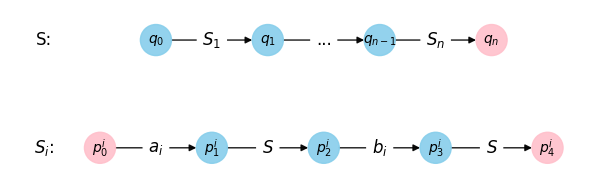
\includegraphics[scale = 0.4]{dyck_n.png}
  \end{center}

  \caption{Possible RSM for Dyck language on $n$ types of brackets. Red vertices $q_n, p^i_4 \; \forall i \in \{1, \ldots, n\}$  are final states, $q_0, p^i_0 \; \forall i \in \{1, \ldots, n\}$ are initial states in each box}

  \label{fig:dyck_n}

\end{figure}

\begin{corollary}
If we fix the input grammar to grammar of Dyck language, then planarity of the Kronecker product is guaranteed if input graph is 1-contractible to a path or is a circuit.
\end{corollary}

\paragraph{Necessary conditions for planarity of Kronecker product of digraphs}

Let us consider the case of product of two planar digraphs. From ~\citep{farzan1977kronecker} it is known, that Kronecker product of $K_{1, 3}$ with itself if non-planar.

\begin{proposition}
If $G_1$ and $G_2$ contain subraphs $K_{1, 3}$ oriented as in Fig.~\ref{fig:k13_0}, ~\ref{fig:k13_3}, ~\ref{fig:k13_12} or ~\ref{fig:k13_21}, then their Kronecker product is non-planar. 
\end{proposition}

$\square$
Proof is a brute-force algorithm that checks planarity of Kronecker product for all possible orientations of pairs of graphs $K_{1, 3}$.

If graphs $G_1$ and $G_2$ contain pair of subgraphs $K_{1, 3}$ which Kronecker product is non-planar, then $G_1 \wedge G_2$ is non-planar too.
$\hfill\blacksquare$

\begin{figure}[h]

  \begin{center}  
  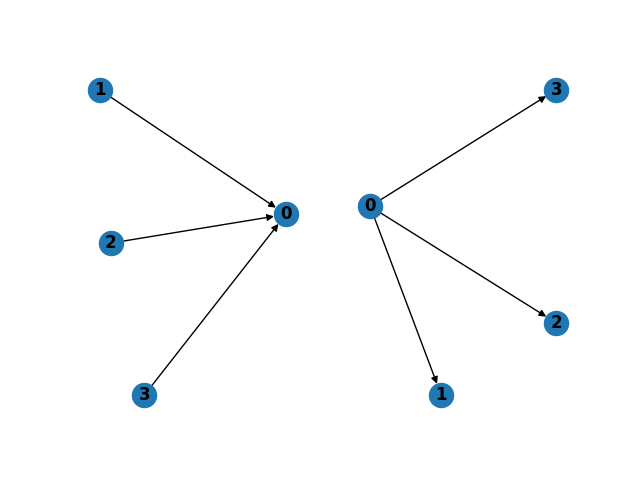
\includegraphics[scale = 0.3]{k13_0.png}
  \end{center}

  \caption{Orientation of the edges of $K_{1, 3}$ graphs, which Kronecker product is non-planar: all edges of the graph at the right are oriented from vertex $0$}

  \label{fig:k13_0}

\end{figure}


\begin{figure}[h]

  \begin{center}  
  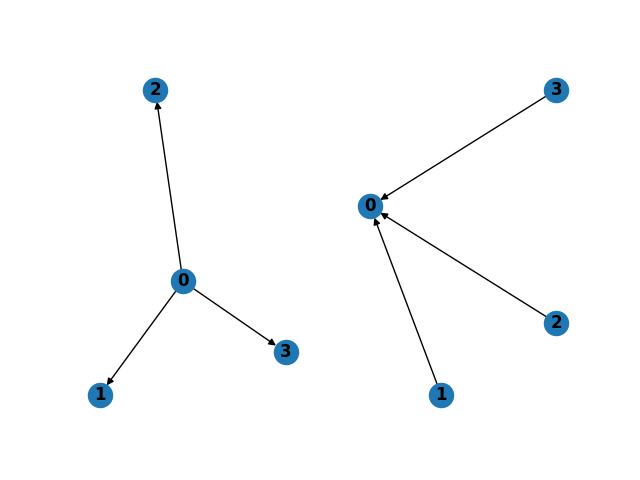
\includegraphics[scale = 0.3]{k13_3.png}
  \end{center}

  \caption{Orientation of the edges of $K_{1, 3}$ graphs, which Kronecker product is non-planar: all edges of the right graph are oriented to vertex $0$}

  \label{fig:k13_3}

\end{figure}

\begin{figure}[h]

  \begin{center}  
  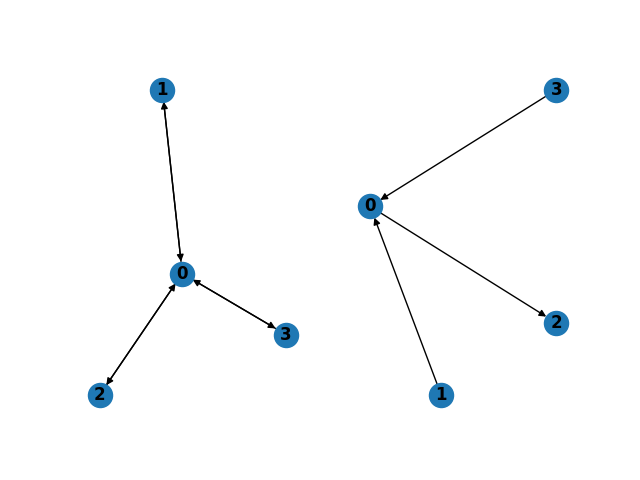
\includegraphics[scale = 0.3]{k13_12.png}
  \end{center}

  \caption{Orientation of the edges of $K_{1, 3}$ graphs, which Kronecker product is non-planar: edges of the right graph are oriented 2 to vertex $0$ and 1 from it}

  \label{fig:k13_12}

\end{figure}

\begin{figure}[h]

  \begin{center}  
  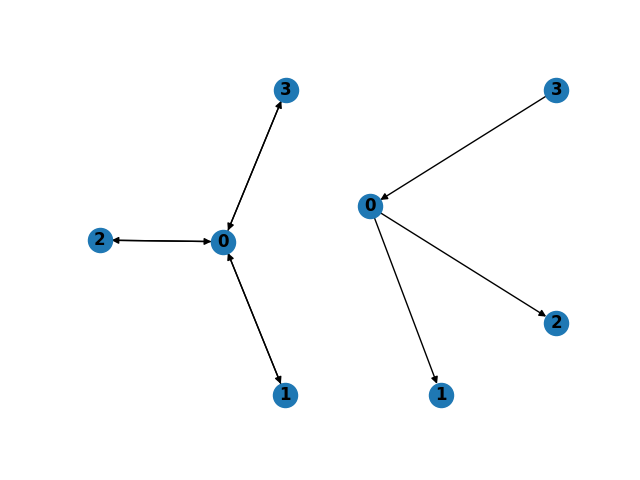
\includegraphics[scale = 0.3]{k13_21.png}
  \end{center}

  \caption{Orientation of the edges of $K_{1, 3}$ graphs, which Kronecker product is non-planar: edges of the right graph are oriented 1 to vertex $0$ and 2 from it}

  \label{fig:k13_21}

\end{figure}
\section{Conclusion and future work}
In this paper, we shown how the context-free path query evaluation w.r.t. the relational and the single-path query semantics can be reduced to the calculation of matrix transitive closure. Also, we provided a formal proof of the correctness of the proposed reduction. In addition, we introduced an algorithm for computing this transitive closure, which allows us to efficiently apply GPGPU computing techniques. Finally, we shown the practical applicability of the proposed algorithm by running different implementations of our algorithm on real-world data.

We can identify several open problems for further research. In this paper we have considered only two semantics of context-free path querying but there are other important semantics, such as all-path query semantics~\cite{hellingsPathQuerying} which requires to present all paths for all triples $(A,m,n)$. Context-free path querying implemented with algorithm~\cite{GLL} can answer the queries in all-path query semantics by constructing a parse forest. It is possible to construct a parse forest for a linear input by matrix multiplication~\cite{okhotin_cyk}. Whether it is possible to generalize this approach for a graph input is an open question.

In our algorithm, we calculate the matrix transitive closure naively, but there are algorithms for the transitive closure calculation, which are asymptotically more efficient. Therefore, the question is whether it is possible to apply these algorithms for the matrix transitive closure calculation to the problem of context-free path querying.

Also, there are Boolean grammars~\cite{okhotinBoolean}, which have more expressive power than context-free grammars. Boolean path querying is an undecidable problem~\cite{hellingsRelational} but our algorithm can be trivially generalized to work on boolean grammars because parsing with boolean grammars can be expressed by matrix multiplication~\cite{okhotin_cyk}. It is not clear what a result of our algorithm applied to Boolean grammars would look like. Our hypothesis is that it would produce the upper approximation of a solution.

From a practical point of view, matrix multiplication in the main loop of the proposed algorithm may be performed on different GPGPU independently. It can help to utilize the power of multi-GPU systems and increase the performance of context-free path querying.

There is an algorithm~\cite{apspGPU} for transitive closure calculation on directed graphs which generalized to handle graph sizes inherently larger then the DRAM memory available on the GPU. Therefore, the question is whether it is possible to apply this approach to the matrix transitive closure calculation in the problem of context-free path querying.



%%
%% The next two lines define the bibliography style to be used, and
%% the bibliography file.
\bibliographystyle{ACM-Reference-Format}
\bibliography{references}

\end{document}
\endinput
%%
%% End of file `sample-sigconf.tex'.
